\documentclass[10pt]{article}
\usepackage{fullpage}
\usepackage{graphicx}
\usepackage{float}
\usepackage{amsmath, amsfonts}
\usepackage[utf8]{inputenc}
\usepackage{parskip}

\usepackage{listings}
\usepackage{color}

%New colors defined below
\definecolor{codegreen}{rgb}{0,0.6,0}
\definecolor{codegray}{rgb}{0.5,0.5,0.5}
\definecolor{codepurple}{rgb}{0.58,0,0.82}
\definecolor{backcolour}{rgb}{0.95,0.95,0.92}

%Code listing style named "mystyle"
\lstdefinestyle{mystyle}{
  backgroundcolor=\color{backcolour},   commentstyle=\color{codegreen},
  keywordstyle=\color{magenta},
  numberstyle=\tiny\color{codegray},
  stringstyle=\color{codepurple},
  basicstyle=\footnotesize,
  breakatwhitespace=false,         
  breaklines=true,                 
  captionpos=b,                    
  keepspaces=true,                 
  numbers=left,                    
  numbersep=5pt,                  
  showspaces=false,                
  showstringspaces=false,
  showtabs=false,                  
  tabsize=2
}


\begin{document}
\begin{center}
{{\Large \sc Algorithms and Data Structures 02105+02326}}
\end{center}
\rule{\textwidth}{1pt}
\begin{description}
\item[Student name and id:] Roar Nind Steffensen (s144107)
\item[Teaching assistant:] Martin Hemmingsen
\item[Hand-in for week:] 8
\end{description}

\section*{Exercise M1}

The floor plan can be represented by a non-directional graph with each room as a node, and each door as an edge between the corresponding nodes.

\section*{Exercise M2}

The given floor plan is shown as a graph in figure \ref{fig:floorplan}

\begin{figure}[H]
    \centering
    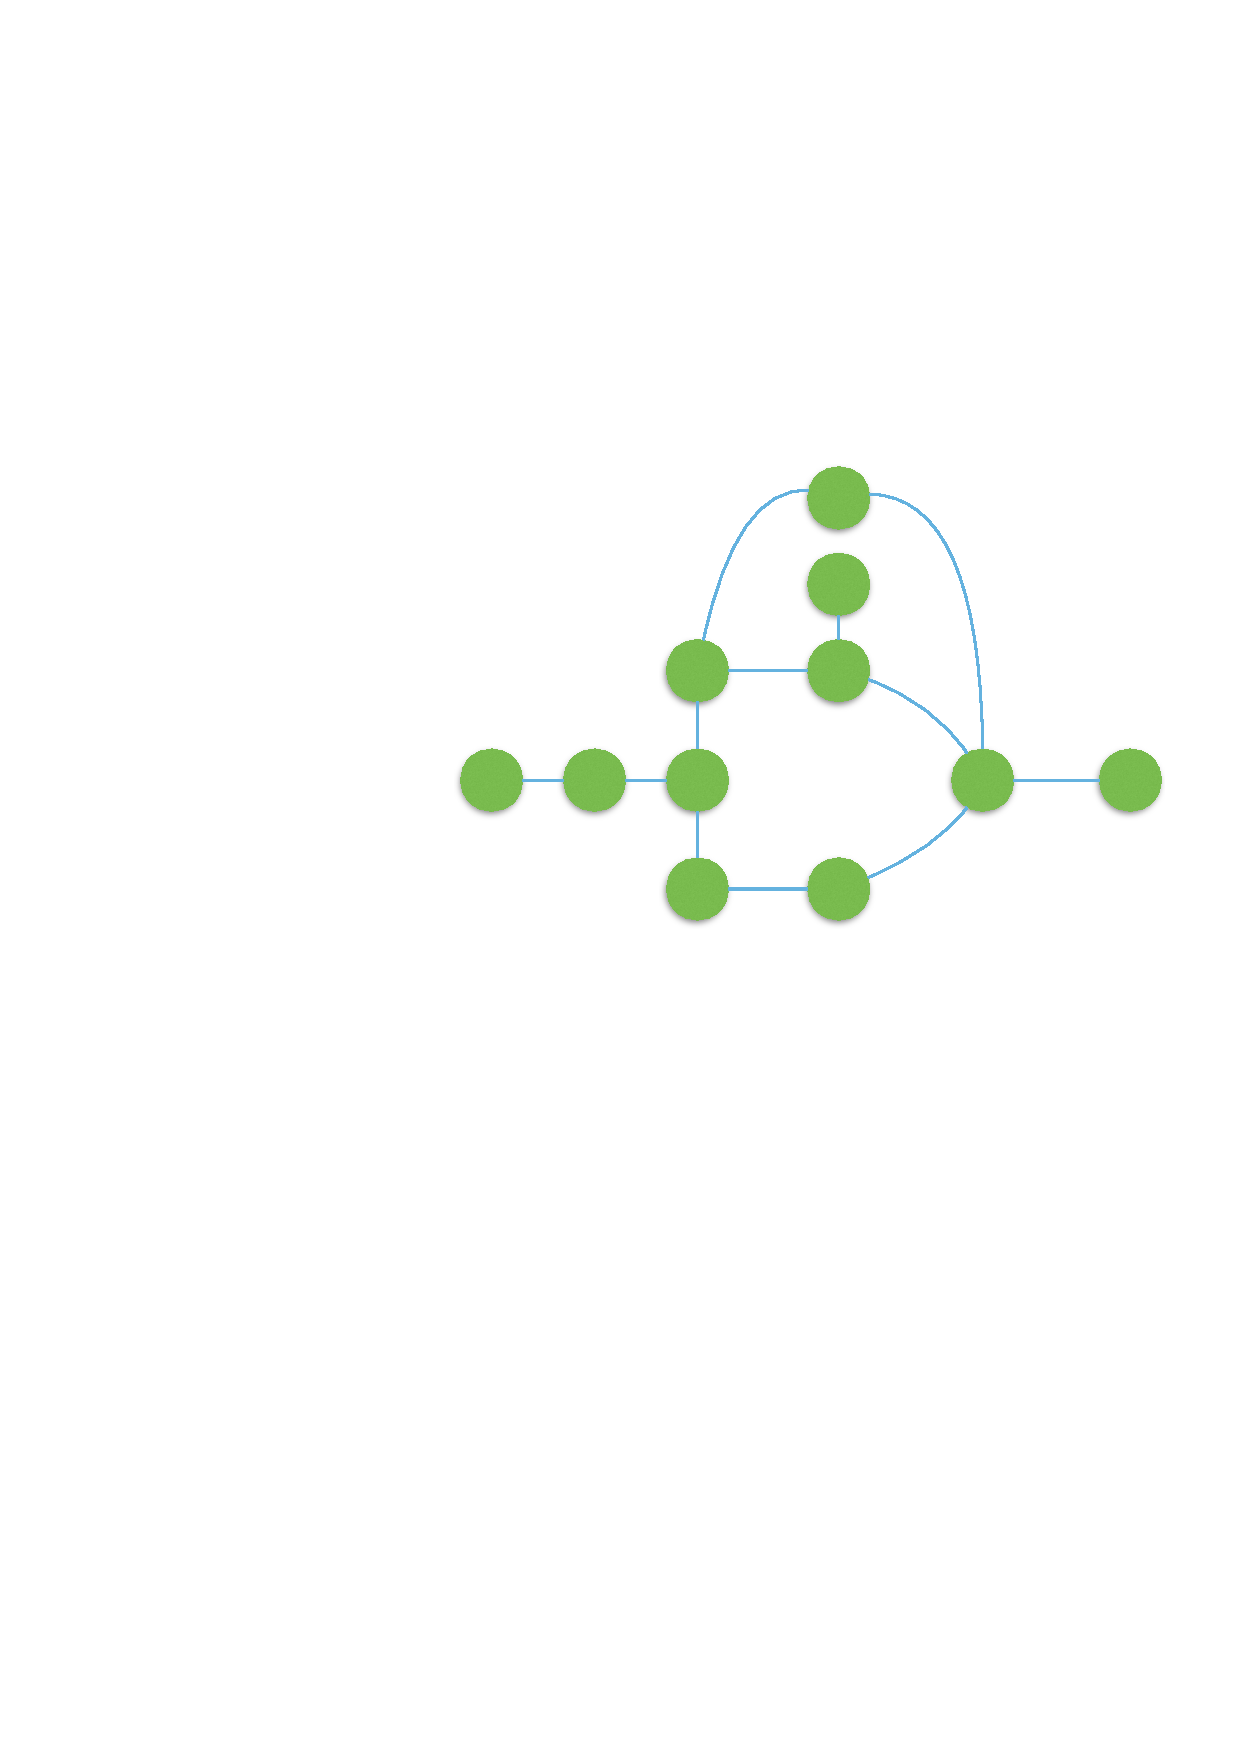
\includegraphics[width=0.4\textwidth]{floorplan}
    \caption{Given example of a floor plan shown as a graph.}
    \label{fig:floorplan}
\end{figure}

\section*{Exercise M3}

In order to check if all rooms can be evacuated, there must exist a path from the room to the entrance $e$. First all fire doors may not be used. The algorithm must remove all edges which is a fire door. This takes $k$ time. Then a recursive check from the entrance $e$ is performed, marking all rooms reachable (marking unmarked children recursively). Then running through the graph's nodes and checking if any of the nodes are unmarked. The result is a time complexity of $\Theta(k+|D| + |R|)$. This algorithm uses a data structure like an array list, with $|R|$ elements containing pointers corresponding to the edges in the graph, and a list of $k$ tuples containing information of which two nodes share a fire door.

\section*{Exercise M4}

As seen on figure \ref{fig:sculptureorpainting} it is possible to make all routes starting and ending in the leftmost room alternate between rooms with sculptures and rooms with paintings. 

\begin{figure}[H]
    \centering
    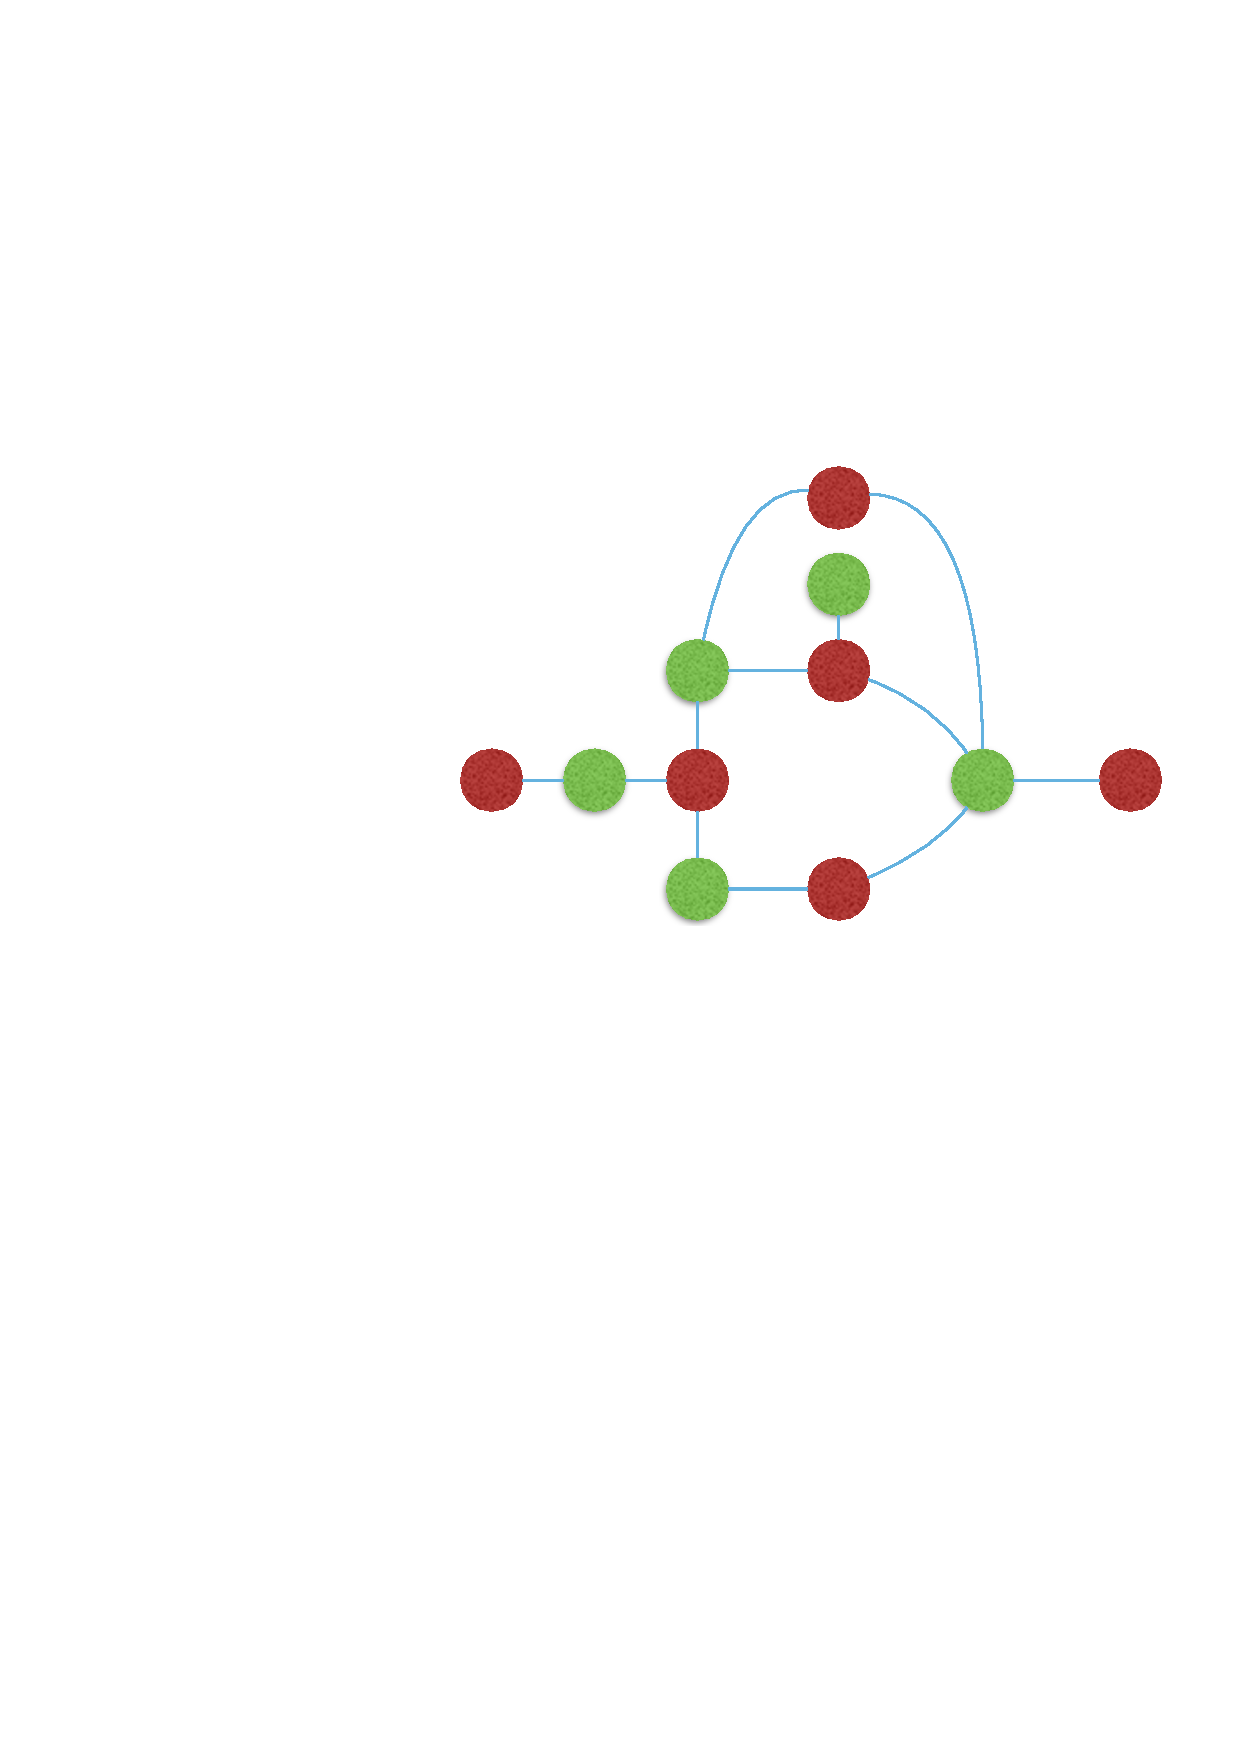
\includegraphics[width=0.5\textwidth]{floorplanSP}
    \caption{Alternating rooms with sculptures and paintings. Green: sculptures, red: paintings.}
    \label{fig:sculptureorpainting}
\end{figure}



\section*{Exercise M5}

An algorithm checking if the route is beautiful is equivalent to checking if the graph is bipartite. To do this BFS is run from the entrance $e$ checking if any room has door to a room with the same interior as itself, or more formally, if a node as an edge to a node with the same property. The time complexity is the same as BFS $\Theta(|R| + |D|)$. 

\end{document}